\chapter{รายละเอียดการปฏิบัติงาน}
\label{chapter:related-theory}

เริ่มสหกิจศึกษาโดยปฏิบัติงานที่ บริษัท วงใน มีเดีย จำกัด (สำนักงานใหญ่) ตั้งแต่วันที่ 4 มิถุนายน พ.ศ.2562 จนถึง 29 พฤศจิกายน พ.ศ.2562 รวมเป็นระยะเวลาประมาณ 6 เดือน โดยในการปฏิบัติงานต่าง ๆ ในช่วงสหกิจศึกษา มีรายละเอียดดังต่อไป

\section{ตำแหน่ง/หน้าที่ของงานที่ได้รับมอบหมาย}
ปฏิบัติงานด้วยตำแหน่ง Software Engineer (Backend) ทำหน้าที่รับผิดชอบในการพัฒนาและดูแลเซิร์ฟเวอร์ของเว็บไซต์ wongnai.com เพื่อให้ผู้ใช้งานทุกแพลตฟอร์มทั้งเว็บไซต์และ แอปพลิเคชันมือถือสามารถทำงานร่วมกันได้อย่างมีประสิทธิภาพ, ควบคุมคุณภาพของโค้ดให้มีคุณภาพที่ดี, ทำงานได้ถูกต้อง, ทดสอบและดูแลได้ง่าย, มีความยืดหยุ่นพร้อมรับการเปลี่ยนแปลงในอนาคต

\section{รายละเอียดของโครงงานที่รับผิดชอบ}
โครงงานที่รับผิดชอบคือ ระบบจัดการโฆษณาแบบจำกัดจำนวนการคลิกและการแสดงโฆษณา เป็นระบบที่พัฒนาขึ้นมาใหม่ต่อจากระบบเดิม ซึ่งจะทำให้ลูกค้าสามารถลงโฆษณากับทาง Wongnai แบบจำกัดจำนวนการแสดงผลและการคลิก อีกทั้งยังสามารถส่งอีเมลรายงานผลการโฆษณากลับไปยังลูกค้าทุก ๆ สัปดาห์โดยอัตโนมัติอีกด้วย

\section{รายละเอียดของงานที่ปฏิบัติ}
ในการปฏิบัติงานครั้งนี้ได้ทำการพัฒนาระบบจัดการโฆษณาแบบจำกัดจำนวนการคลิกและการแสดงโฆษณาเฉพาะฟังก์ชันหลักที่จำเป็น เพื่อให้สามารถส่งมอบงานได้เร็วที่สุดและสามารถทำงานได้เป็นระบบ ได้แก่ ฟังก์ชันการจำกัดการแสดงโฆษณาของร้านด้วยจำนวนการคลิกโฆษณา กับฟังก์ชันการส่งอีเมลรายงานผลการโฆษณากลับไปยังลูกค้าโดยอัตโนมัติทุก ๆ สัปดาห์ โดยในการปฏิบัติงานครั้งนี้ เพื่อให้การพัฒนาระบบเป็นไปอย่างราบรื่น, รวดเร็ว และสามารถทำงานร่วมสมาชิกทีมคนอื่น ๆ ได้อย่างมีประสิทธิภาพ จึงได้มีการนำเทคโนโลยีและเครื่องมือต่าง ๆ มาใช้งาน ได้แก่
\begin{enumerate}
	\item IntelliJ IDEA
	
	IntelliJ IDEA เป็น Integrate Development Environment (IDE) สำหรับใช้ในการพัฒนาซอฟต์แวร์ที่ใช้ Java Virtual Machine (JVM) โดยเฉพาะ มีระบบแนะนำการเขียนโค้ดที่ทำให้การเขียนโค้ดเป็นไปอย่างราบรื่นและรวดเร็ว ~\cite{intellij}
	\item Sequel Pro
	
	Sequel Pro เป็นแอปพลิเคชันสำหรับจัดการฐานข้อมูล MySQL ~\cite{sequelpro}
	\item Postman
	
	Postman เป็นแอปพลิเคชันสำหรับสร้าง API Request เช่น REST, SOAP, GraphQL เพื่อทดสอบการทำงาน API ของ Server และสามารถตรวจสอบ Response ที่ส่งกลับมาได้ ~\cite{postman}
	\item Visual Studio Code
	
	Visual Studio Code เป็น Text Editor ที่รองรับได้หลากหลายภาษา มีระบบไฮไลท์ Syntax ในการตรวจสอบ Syntax ของโค้ด และสามารถติดตั้งส่วนขยายต่าง ๆ เพิ่มเติมได้ตามความเหมาะสมในการทำงาน ~\cite{vscode}
	\item GitKraken
	
	GitKraken เป็น Git GUI Client ที่ทำให้สามารถใช้งาน Git ได้อย่างสะดวกสบาย ~\cite{gitkraken}
	\item Asana
	
	Asana คือระบบออนไลน์ที่คอยแสดงสถานะการทำงานของสมาชิกทีม ทำให้สมาชิกคนอื่น ๆ ในทีมสามารถทราบสถานะงานของแต่ละคนได้อย่างรวดเร็ว ~\cite{asana}
	\item Java
	
	Java เป็นภาษาคอมพิวเตอร์ประเภท Object-Oriented เมื่อคอมไพล์แล้วจะได้ bytecode โดยเราสามารถนำ bytecode นี้ ไปใช้งานบนคอมพิวเตอร์เครื่องไหนก็ได้ที่มี Java Virtual Machine (JVM) ~\cite{java}
	\item Python
	
	Python เป็นภาษาคอมพิวเตอร์ระดับสูงที่ใช้ Python Interpreter มีจุดเด่นที่สามารถอ่านและทำความเข้าใจโค้ดได้ง่าย โดย Python Interpreter นั้น สามารถติดตั้งได้ในหลากหลายระบบปฏิบัติการ  ~\cite{python}	
	\item MySQL
	
	MySQL เป็นตัวจัดการฐานข้อมูลแบบ Relational ที่เป็น Open source ~\cite{mysql}
	\item Google BigQuery
	
	Google BigQuery เป็นบริการคลังข้อมูลบน Cloud ที่ให้บริการโดย Google และสามารถใช้ SQL เพื่อใช้งาน Google BigQuery ได้ ~\cite{bigquery}
	\item Git
	
	Git คือ Version Control ที่สามารถติดตามและควบคุมการเปลี่ยนแปลงของโค้ดได้ เพื่อให้ Software Engineer คนอื่น ๆ สามารถทำงานร่วมกันได้อย่างมีประสิทธิภาพ ~\cite{git}
	\item Spring Boot
	
	Spring Boot คือ เฟรมเวิร์คสำหรับพัฒนา REST API, Websocket, Web และอื่น ๆ ของภาษาที่ใช้ Java Virtual Machine (JVM) ~\cite{spring}
	\item Docker
	
	Docker คือ เทคโนโลยีสำหรับสร้างคอนเทนเนอร์ของซอฟต์แวร์ ทำให้ซอฟต์แวร์สามารถนำไปใช้งานในสภาพแวดล้อมไหนก็ได้ ~\cite{docker}
	\item Kubernetes

	Kubernetes คือ เทคโนโลยีสำหรับจัดการกลุ่มเครื่องเซิร์ฟเวอร์ มีความสามารถในการจัดการเซิร์ฟเวอร์ให้สามารถทำงานได้อย่างต่อเนื่อง มีจุดเด่นในการทำให้มีช่วงเวลาที่เซิร์ฟเวอร์หยุดทำงานเป็นศูนย์ ~\cite{kubernetes}
	\item Gitlab CI/CD
	
	Gitlab CI/CD คือ เครื่องมือในการ Build ซอฟต์แวร์และ Deploy โดยอัตโนมัติ ~\cite{gitlabcicd}
\end{enumerate}

\begin{figure}[!h]
	\centering
	\subfigure[]{
		\label{Fig:technology:intellij}
		
\includegraphics[width=0.15\textwidth]{intellij}  
	}
	\subfigure[]{
		\label{Fig:technology:sequelpro}
		
\includegraphics[width=0.15\textwidth]{sequelpro}  
	}
	\subfigure[]{
		\label{Fig:technology:postman}
		
\includegraphics[width=0.15\textwidth]{postman}  
	}
	\subfigure[]{
		\label{Fig:technology:vscode}
		
\includegraphics[width=0.15\textwidth]{vscode}  
	}
	\subfigure[]{
		\label{Fig:technology:gitkraken}
		
\includegraphics[width=0.15\textwidth]{gitkraken}  
	}
	\subfigure[]{
		\label{Fig:technology:asana-icon}
		
\includegraphics[width=0.15\textwidth]{asana-icon}  
	}
	\subfigure[]{
	\label{Fig:technology:java}
	
\includegraphics[width=0.15\textwidth]{java}  
	}
	\subfigure[]{
		\label{Fig:technology:python}
		
\includegraphics[width=0.15\textwidth]{python}  
	}
	\subfigure[]{
		\label{Fig:technology:mysql}
		
\includegraphics[width=0.25\textwidth]{mysql}  
	}
	\subfigure[]{
		\label{Fig:technology:bigquery}
		
\includegraphics[width=0.25\textwidth]{bigquery}  
	}
	\subfigure[]{
		\label{Fig:technology:git}
		
\includegraphics[width=0.15\textwidth]{git}  
	}
	\subfigure[]{
		\label{Fig:technology:spring-boot}
		
\includegraphics[width=0.15\textwidth]{spring-boot}  
	}
	\subfigure[]{
		\label{Fig:technology:docker}
		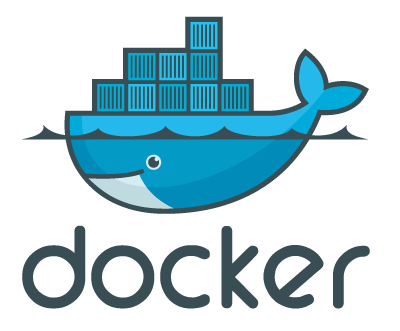
\includegraphics[width=0.15\textwidth]{docker}  
	}
	\subfigure[]{
		\label{Fig:technology:k8s}
		
\includegraphics[width=0.25\textwidth]{k8s}  
	}
	\subfigure[]{
		\label{Fig:technology:gitlab-ci-cd}
		
\includegraphics[width=0.15\textwidth]{gitlab-ci-cd}  
	}
	\caption{สัญลักษณ์ของเทคโนโลยีและเครื่องมือต่าง ๆ ที่ใช้ IntelliJ IDEA (ก), Sequel Pro (ข), Postman (ค), Visual Studio Code (ง), GitKraken (จ), Asana (ฉ), Java (ช), Python (ซ), MySQL (ฌ), Google BigQuery (ญ), Git (ฎ), Spring Boot (ฏ), Docker (ฐ), Kubernetes (ฑ), Gitlab CI/CD (ฒ)}
	\label{Fig:technology}
\end{figure}

ระบบจัดการโฆษณาแบบจำกัดจำนวนการคลิกและการแสดงโฆษณาที่พัฒนาขึ้นมานั้น ประกอบด้วยเซอร์วิสต่าง ๆ ได้แก่

\begin{figure}[!h]
	\centering
	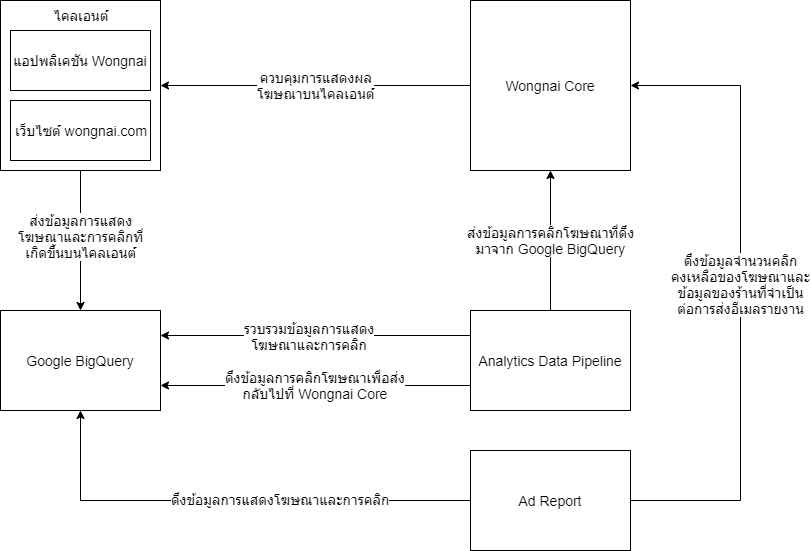
\includegraphics[width=1\textwidth]{ad-report-diagram.png}  
	\caption{แผนผังภาพรวมการทำงานของระบบจัดการโฆษณาแบบจำกัดจำนวนการคลิกและการแสดงโฆษณา}
	\label{Fig:adreport-diagram}
\end{figure}

\begin{enumerate}
	\item Wongnai Core
	
	Wongnai Core เป็นเซอร์วิสหลักของ Wongnai ถูกพัฒนาด้วยภาษา Java ทำหน้าที่ให้บริการหลาย ๆ อย่าง โดยหน้าที่ของ Wongnai Core ที่เกี่ยวข้องกับระบบจัดการโฆษณาแบบจำกัดจำนวนการคลิกและการแสดงโฆษณา ได้แก่ 
	\begin{itemize}
		\item[-] ควบคุมการแสดงผลโฆษณาของเว็บไซต์ wongnai.com และแอปพลิเคชัน Wongnai
		\item[-] รับข้อมูลจำนวนคลิกของโฆษณา เพื่อนำมาอัปเดตในฐานข้อมูลของ Wongnai Core จากนั้นจึงทำการประมวลผลและพิจารณาว่าควรจะนำโฆษณาที่แสดงอยู่ออกหรือไม่ โดยดูจากจำนวนคลิกของโฆษณาว่าเกินกว่าที่จำกัดไว้ตามที่ตกลงกันหรือไม่ ถ้าเกินก็จะหยุดการแสดงโฆษณานั้น ๆ
		\item[-] รอรับการร้องขอข้อมูลจากเซอร์วิส Ad Report เพื่อนำข้อมูลไปใช้ในการสร้างรายงานที่สมบูรณ์ส่งกลับไปยังเจ้าของโฆษณา ซึ่งประกอบไปด้วย ชื่อร้าน, อีเมลของร้าน, จำนวนคลิกโฆษณาของร้านที่ใช้ไปแล้ว และจำนวนคลิกโฆษณาของร้านซื้อไว้
	\end{itemize}
	\item Analytics Data Pipeline
	
	Analytics Data Pipeline เป็นเซอร์วิสขนาดเล็กที่ถูกพัฒนาด้วยภาษา Python ปกติแล้วไคลเอนต์จะส่งข้อมูลเหตุการณ์ต่าง ๆ ที่เกิดขึ้นใน Wongnai มาเก็บใน Google BigQuery ซึ่งข้อมูลเหตุการณ์ต่าง ๆ นั้นมีหลากหลายมาก โดยข้อมูลที่จำเป็นต้องใช้เพื่อให้แสดงโฆษณาแบบจำกัดจำนวนการคลิกได้ ได้แก่ ข้อมูลที่ผู้ใช้ Wongnai ที่คลิกไปยังโฆษณา ซึ่งข้อมูลเหตุการณ์ที่เกิดขึ้นใน Wongnai ทุก ๆ อย่างนั้นจะถูกเก็บอยู่ในตารางข้อมูลเดียวกันทั้งหมด ทำให้ตารางนั้นเป็นตารางที่มีข้อมูลมหาศาล และการดึงข้อมูลจาก Google BigQuery หนึ่งครั้งจะต้องเสียเครดิตตามขนาดของข้อมูลในตาราง หากดึงจากตารางขนาดใหญ่นั้นโดยตรง จะทำให้สูญเสียเครดิตไปโดยไม่จำเป็น Analytics Data Pipeline จึงถูกพัฒนาขึ้นเพื่อแก้ไขปัญหาในจุดนี้ โดยเซอร์วิสนี้จะทำการใช้คำสั่ง SQL เพื่อสร้างตารางข้อมูลใหม่โดยแยกออกมาจากตารางขนาดใหญ่อีกที และรวบรวมข้อมูลเฉพาะส่วนที่ต้องการมาเก็บไว้ ทำให้ได้ตารางข้อมูลที่มีขนาดเล็กลง และมีเฉพาะส่วนที่เราต้องการนำไปใช้จริง ๆ โดยในที่นี้เราจะแยกเฉพาะข้อมูลการแสดงโฆษณาของ Wongnai และข้อมูลที่ผู้ใช้ Wongnai ที่คลิกไปยังโฆษณา หน้าที่อีกอย่างหนึ่งที่สำคัญของเซอร์วิสนี้ คือการนำข้อมูลการคลิกของโฆษณาที่รวมรวบไปเก็บในตารางขนาดเล็กแล้ว ส่งไปอัปเดตที่ฐานข้อมูลของ Wongnai Core ทุก ๆ วัน เพื่อให้ Wongnai Core นำข้อมูลส่วนนี้ไปประมวลผลต่อ

	\item Ad Report
	
	Ad Report เป็นเซอร์วิสใหม่ที่ถูกพัฒนาด้วยภาษา Java ร่วมกับ Spring Boot ทำหน้าที่สร้างอีเมลรายงานสถิติของโฆษณาที่ประกอบไปด้วยข้อมูลต่าง ๆ เช่น จำนวนการแสดงผลโฆษณาต่อวัน, จำนวนผู้ที่คลิกเข้าไปในโฆษณาต่อวัน, จำนวนการคลิกของโฆษณาที่ยังคงเหลือ และจำนวนคลิกของโฆษณาที่ลูกค้าซื้อไว้ เป็นต้น โดยภายในเซอร์วิสนี้ จะมีฟังก์ชันการทำงานหลัก 4 อย่าง ได้แก่
	\begin{itemize}
		\item Statistics Updater
		
		 ฟังก์ชัน Statistics Updater ทำหน้าที่นำข้อมูลของโฆษณาจาก Google BigQuery มาอัปเดตในฐานข้อมูลของ Ad Report กรณีที่ข้อมูลที่เข้ามาเป็นของร้านที่ไม่เคยปรากฏอยู่ในฐานข้อมูลของ Ad Report (เป็นร้านที่ลงโฆษณากับ Wongnai เป็นครั้งแรก) ก็จะทำการเรียกฟังก์ชัน Retrieve Data เพื่อร้องขอข้อมูลจาก Wongnai Core ซึ่งประกอบไปด้วยชื่อร้าน และอีเมลของร้าน นำไปประกอบในการทำรายงานที่สมบูรณ์และส่งอีเมลกลับไปได้
		\item Report
		
		ฟังก์ชัน Report ทำหน้าที่สร้างรายงานที่จะส่งไปพร้อมกับอีเมลให้กับลูกค้า
		\item Report Email
		
		ฟังกชัน Report Email ทำหน้าที่สร้างอีเมลพร้อมกับแนบไฟล์รายงานที่ได้จากฟังก์ชัน Report ส่งไปยังอีเมลของลูกค้า
		\item Retrieve Data
		
		ฟังกชัน Retrieve Data ทำหน้าหน้าที่ร้องขอข้อมูลที่จำเป็นจาก Wongnai Core โดยใช้โปรโตคอล HTTP เพื่อนำไปใช้ในการสร้างรายงานและการส่งอีเมลที่สมบูรณ์
	\end{itemize}
	โดยภายใน Ad Report จะมี Cron ซึ่งเป็นเครื่องมือของ Unix ที่จะทำให้สามารถรัน Command Line หรือ Shell Scripts ตามช่วงเวลาที่เรากำหนดไว้ได้โดยอัตโนมัติ ในที่นี้ได้มีการนำ Cron ไปใช้งาน 2 ส่วน ได้แก่
	\begin{itemize}
		\item Daily Statistics Updater
		
		Daily Statistics Updater จะเรียกใช้งานฟังก์ชัน Statistics Updater ทุก ๆ วัน เพื่ออัปเดตฐานข้อมูลของ Ad Report
		\item Weekly Report Email
		
		Weekly Report Email จะเรียกใช้งานฟังก์ชัน Report และ Report Email เพื่อสร้างรายงานสถิติของโฆษณาและส่งอีเมลกลับไปยังลูกค้าทุก ๆ สัปดาห์ ซึ่งจะส่งให้เฉพาะร้านที่ยังจำนวนคลิกโฆษณาคงเหลืออยู่ โดยดูจากข้อมูลที่ร้องขอมาจากฟังก์ชัน Retrieve Data
	\end{itemize}
\end{enumerate}

เซอร์วิสทั้งหมดที่กล่าวมาข้างต้นจะใช้ Docker สร้างอิมเมจของแต่ละเซอร์วิสสำหรับเซอร์วิส และเซิร์ฟเวอร์ที่รันคอนเทนเนอร์ของอิมเมจของแต่ละเซอร์วิสจะถูกจัดการด้วย Kubernetes ทั้งหมด
\begin{figure}[!h]
	\centering
	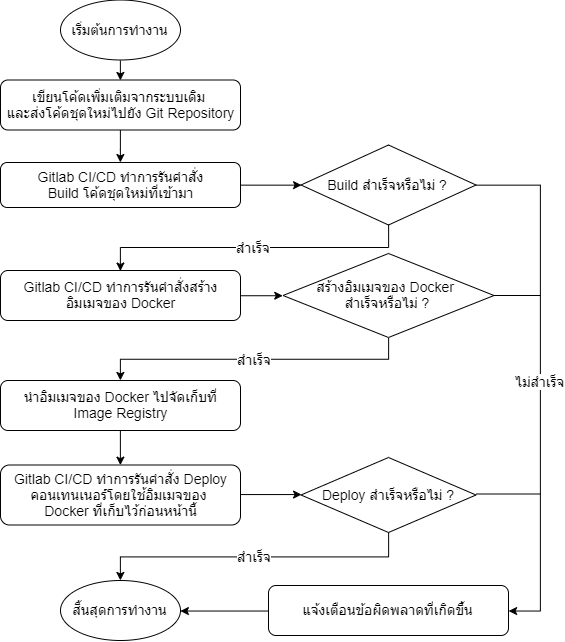
\includegraphics[width=0.9\textwidth]{gitlab-flow.png}  
	\caption{แผนผังวิธีการ Deploy โค้ดชุดใหม่ของเซอร์วิส Ad Report}
	\label{Fig:adreport-diagram}
\end{figure}

สำหรับ Ad Report ซึ่งเป็นเซอร์วิสใหม่นั้น ได้ทำการเพิ่มสคริปสำหรับใช้งาน Gitlab CI/CD เพื่อให้ทำการ Build โค้ด, สร้างอิมเมจ Docker, นำไปจัดเก็บใน Image Registry ที่เป็นพื้นที่สำหรับจัดเก็บอิมเมจ และ Deploy เซอร์วิสโดยอัตโนมัติ การนำอิมเมจ Docker ที่ได้ไป Deploy เป็นคอนเทนเนอร์บนเครื่องเซิร์ฟเวอร์จะมี Project Eastern ซึ่งเป็นไลบรารีที่ช่วย Deploy คอนเทนเนอร์บน Kubernetes และช่วยจัดการ Environment ที่จะ Deploy ให้ ~\cite{eastern} 

\section{ลักษณะขั้นตอนการทำงาน}
ทีม Development ของบริษัท วงใน มีเดีย จำกัด (สำนักงานใหญ่) จะถูกแบ่งออกเป็นทีมย่อย ๆ ตามประเภทของงานที่รับผิดชอบ เรียกว่า Squad ซึ่งจะเป็นทีมแบบ Cross-Functional กล่าวคือ ภายในทีมจะประกอบไปด้วยหลาย ๆ ฝ่าย ได้แก่ Project Manager, UX/UI Designer, Software Engineer (Frontend), Software Engineer (Backend), Software Engineer (iOS), Software Engineer (Android) และ Quality Assurance Engineer โดยแต่ละ Squad อาจจะฝ่ายอื่น ๆ เพิ่มเติมแตกต่างกันไป ขึ้นอยู่กับลักษณะของงานที่รับผิดชอบ โดยแต่ละ Squad นั้นจะทำงานโดยใช้ Scrum Framework เป็นหลัก Scrum จะทำงานเป็นวงรอบ (Sprint) แต่ละรอบนั้นจะเท่ากับ 2 สัปดาห์ ภายใน Sprint จะกิจกรรมที่สำคัญต่าง ๆ ดังต่อไปนี้
\begin{enumerate}
	\item Sprint Planning
	
	เป็นการประชุมตอนต้น Sprint เพื่อรับมอบหมายงานจาก Project Manager และเป็นการประชุมเพื่อปรึกษาหาวิธีการทำงานและวิธีการแก้ไขปัญหาต่าง ๆ ที่เกี่ยวกับงานที่ได้รับมอบหมาย
	
	\item Daily Meeting
	
	เป็นการประชุมแบบสั้น ๆ ประจำวัน มีจุดประสงค์เพื่อให้สมาชิกทีมรับทราบความคืบหน้าของงานที่แต่ละคนกำลังทำอยู่และทราบปัญหาที่เกิดขึ้นระหว่างการทำงาน
	
	\item Backlog Refinement Meeting
	
	ปกติเมื่อ Squad ได้รับมอบหมายให้ทำงานใหม่ ๆ งานนั้นจะถูกจัดไว้ใน Features Backlog ก่อน ซึ่งงานที่อยู่ในนี้จะถูกนำเข้า Sprint ถัด ๆ ไป ขึ้นอยู่กับการตัดสินใจของ Project Manager การประชุมนี้จะจัดตอนกลาง Sprint เพื่อพิจารณางานที่อยู่ Features Backlog ว่าควรจะทำอย่างไร, เป็นงานสำคัญที่ต้องเอามาเท่าก่อนหรือไม่ และประเมินเวลาที่จะต้องใช้ในการทำงานชิ้นนี้ เป็นต้น
	
	\item Retrospective Meeting
	
	เป็นการประชุมตอนปลาย Sprint เพื่อสรุปการทำงานที่ได้ทำไปในรอบ และให้สมาชิกภายในทีมอธิบายปัญหาที่เกิดขึ้นในรอบ รวมไปถึงเรื่องราวดี ๆ ที่เกิดขึ้นในรอบด้วย เพื่อนำไปปรับปรุงการทำงานในรอบถัดไป
\end{enumerate}

การติดต่อสื่อสารภายในองค์กรจะใช้โปรแกรม Slack เป็นหลัก สถานะของงานภายในทีมสามารถดูได้จาก Kanban Board ซึ่งเป็นบอร์ดที่ตั้งอยู่ในพื้นที่ทำงาน และ Asana ซึ่งเป็นระบบออนไลน์ที่จะทำให้สมาชิกภายในทีมสามารถทราบสถานะของงานได้อย่างรวดเร็ว ภายในกระบวนการทำงาน สถานะของงานจะเป็นไปตามดังต่อไปนี้

\begin{enumerate}
	\item To do
	
	งานที่ยังไม่ได้เริ่มทำ แต่อยู่ในรอบแล้วจะมีสถานะเป็น To do
	
	\item In progress
	
	งานที่กำลังทำอยู่จะมีสถานะเป็น In progress
	
	\item Review
	
	เมื่องานที่ทำอยู่เสร็จแล้ว ก่อนที่จะนำงานส่วนที่ทำเข้าไปใน Beta Environment ของเซิฟเวอร์ ซึ่งเป็น Environment ที่มีไว้ทดสอบก่อนที่จะใช้งานจริง โค้ดที่เขียนขึ้นมาจะต้องผ่านการตรวจสอบจาก Software Engineer คนอื่นอย่างน้อย 2 คนก่อน จึงจะสามารถส่งไปให้ Quality Assurance Engineer ทำการทดสอบต่อได้
	
	\item Review passed
	
	เมื่องานที่ทำอยู่ผ่านการตรวจสอบโดย Software Engineer คนอื่นครบ 2 คนแล้ว งานจะอยู่ในสถานะ Review passed 
	
	\item Testing
	งานที่อยู่ในสถานะ Review passed จะถูกส่งต่อให้ Quality Assurance Engineer ทดสอบ ซึ่งก่อนที่จะให้ Quality Assurance Engineer ทดสอบนั้น จะต้องเตรียมวิธีการทดสอบและเตรียมข้อมูลให้เรียบร้อยก่อน
	
	\item Test passed
	
	เมื่อ Quality Assurance Engineer ทดสอบเสร็จแล้ว งานจะอยู่ในสถานะ Test passed สามารถนำงานเข้า Beta Environment ได้เลย
	
	\item Done
	
	เมื่อนำงานเข้าไปใน Beta Environment เสร็จแล้ว งานจะมีสถานะเป็น Done แต่อย่างไรก็ตาม เจ้าของงานจะต้องติดตามงานของตัวเองจนกว่างานจะขึ้นอยู่บนระบบที่ใช้งานจริง (Production Environment)
\end{enumerate}

โดยส่วนมากแล้ว ถ้าเป็นงานที่เป็นการเขียนโค้ดจะมีกระบวนการทำงานตามที่กล่าวมาข้างต้น แต่อย่างไรก็ตามงานบางชนิดไม่จำเป็นต้องทำตามกระบวนการอย่างเคร่งครัดก็ได้ ขึ้นอยู่กับความเหมาะสมของงานว่าควรจะเป็นแบบไหน และในการทำงานของทีม Development ที่เป็นการเขียนโค้ดจะใช้ Test Driven Development (TDD) เป็นหลัก เป็นการเขียนชุดทดสอบของโค้ดขึ้นมาก่อน แล้วรันชุดทดสอบให้เกิดข้อผิดพลาด จากนั้นจึงเขียนโค้ดเพื่อแก้ไขข้อผิดพลาดนั้น ระหว่างการเขียนโค้ดจะต้องคอยคำนึงถึงคุณภาพของโค้ด หากมีโค้ดส่วนที่ไม่จำเป็นกจะต้องทำการ Refactor โค้ดส่วนนั้นด้วย โดยการ Refactor จะเป็นการลบโค้ดส่วนที่ไม่จำเป็นออก และนำโค้ดส่วนอื่น ๆ มาใช้ซ้ำให้มากที่สุด เพื่อให้โค้ดสั้นลง, มีคุณภาพ และ Software Engineer คนอื่น สามารถพัฒนาโค้ดส่วนนี้ต่อได้ง่าย

\begin{figure}[!h]
	\centering
	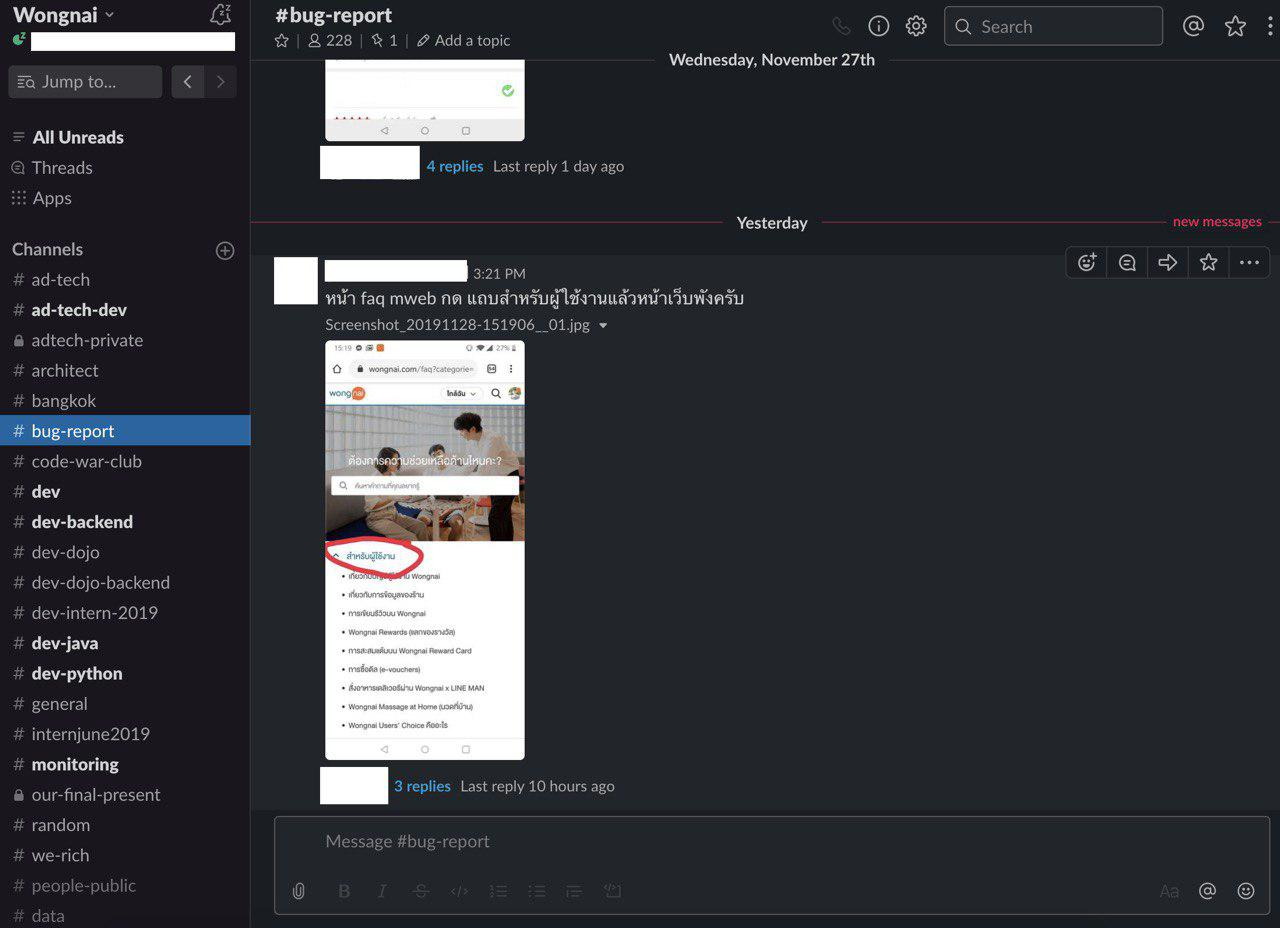
\includegraphics[width=1\textwidth]{slack}  
	\caption{ตัวอย่างของโปรแกรม Slack}
	\label{Fig:slack}
\end{figure}

\begin{figure}[!h]
	\centering
	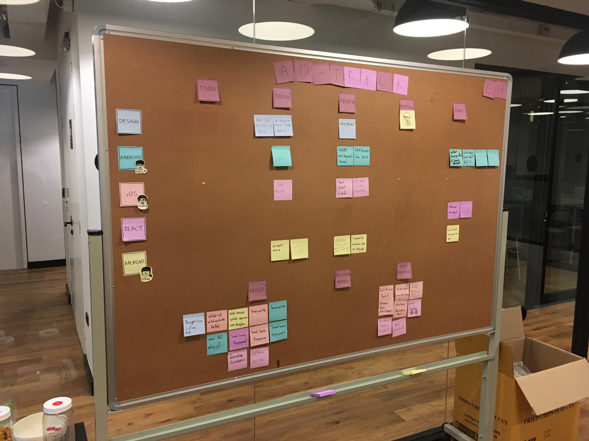
\includegraphics[width=1\textwidth]{kanban-board.png}  
	\caption{Kanban Board ที่ตั้งอยู่ในพื้นที่ทำงาน}
	\label{Fig:kanban-board}
\end{figure}

\begin{figure}[!h]
	\centering
	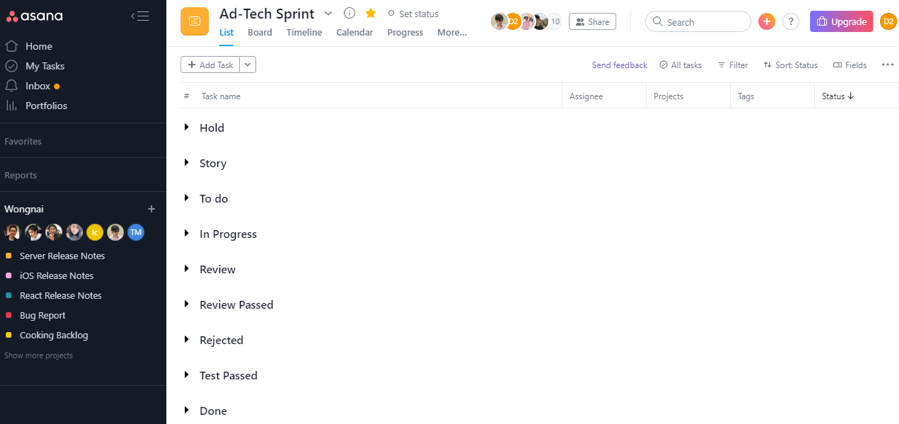
\includegraphics[width=1\textwidth]{asana}  
	\caption{ตัวอย่างของโปรแกรม Asana}
	\label{Fig:asana}
\end{figure}